\documentclass[letterpaper,10pt,spanish,titlepage]{article}

%Configuracion inicial
\PassOptionsToPackage{activeacute}{babel}

% \usepackage{geometry}
\usepackage[]{fontenc}
\usepackage[spanish]{babel}
\usepackage[latin1]{inputenc}
\usepackage{moreverb}
\usepackage{epsfig}
\usepackage{fancyhdr}
\usepackage{multicol}
\usepackage{rotating}
\usepackage{graphics}
\usepackage{graphicx}

\usepackage{float}
\usepackage{textcomp}
\usepackage{alltt}
\usepackage{times}
\usepackage{makeidx}
\usepackage{tocbibind}
\usepackage{array}

\newcommand{\TODO}[0] {
\begin{center}
	\textbf{\underline{\color{red}{Esta secci�n necesita ser completada.}}}
\end{center}
}

\newcommand{\comillas}[1] {
``#1''
}

\newcommand{\nuevo}[1] {
	{\color{magenta}{#1}}
}

\newcommand{\ds}[0] {\\ \\}

\ifx\pdfoutput\undefined
\usepackage[ps2pdf,
            pagebackref=true,
            colorlinks=true,
            linkcolor=blue
           ]{hyperref}
\usepackage{pspicture}
\else
\usepackage[pdftex,
%             pagebackref=true,
            colorlinks=true,
            linkcolor=blue
           ]{hyperref}
\fi

\bibliographystyle{alpha}
% \setcounter{tocdepth}{2}
% \setcounter{secnumdepth}{4}

\pagestyle{fancy}
\fancyhf{}

% configuraci�n del encabezado
\fancyhead[L]{

\includegraphics[width=7cm]{images/header.png}
}

\fancyhead[RO,LE]{\thepage}

% Tama�os
% \setlength{\textwidth}{15cm}
% \setlength{\topmargin}{3cm}
% \setlength{\headheight}{1cm}
% \setlength{\headsep}{0.8cm}
% \setlength{\textheight}{23cm}

%opening
\title
{
  \textsc{Universidad del Valle}\\
  Escuela de Ingenier�a de Sistemas y Ciencias de la Computaci�n \\
  \textbf{Modulo para la creaci�n de producciones de animaci�n mediante un enfoque colaborativo.}
}

\author
{
	David Alejandro Cuadrado Cabrera \\
	Jorge Humberto Cuadrado Cabrera \\
	\\
	\textbf{Directora:} Profesora. Paola Johana Rodriguez
}

\date{\today}

\begin{document}

\maketitle

\begin{abstract}

A continuaci�n se presenta una propuesta de trabajo de grado que trata de solucionar las problem�ticas en la producci�n de animaciones utilizando un enfoque \hyperlink{modelo_colaborativo}{colaborativo} para el proceso de creaci�n de las mismas.

Mediante este enfoque los \hyperlink{director_animacion}{directores de la animaci�n} podr�n ser capaces de fiscalizar el trabajo que lleva a cabo cada animador en la realizaci�n de los diferentes planos de animaci�n, as� como gestionar todo el proceso de producci�n.

A su vez, ser� permitido que dos o m�s animadores interact�en en un mismo \hyperlink{scene}{plano} o \hyperlink{frame}{marco} si es
deseado, contribuyendo as� con mejoras notables en los tiempos de producci�n.

\end{abstract}

\tableofcontents

\section{Introducci�n}
{
	Durante muchos a�os la industria de producci�n de animaciones se ha regido por el proceso de animaci�n cuadro-a-cuadro, el cual se trata de dibujar todos los cuadros que componen la animaci�n, recientemente se han incorporado al proceso algunas t�cnicas avanzadas de interpolaci�n de movimiento que simplifican el proceso.
}


\section{Planteamiento y Formulaci�n del Problema}
{
	\subsection{Planteamiento del problema}
	A grandes rasgos, para crear una producci�n animada lo primero que se necesita es una idea proveniente del creador original, despues de que la idea est� clara es necesario realizar el gui�n de la producci�n, el cual consigna los di�logos y acciones que deben seguir los personajes de la producci�n.
	\ds
	Una vez que se ha dise�ado el gui�n, un miembro de la productora se encarga de realizar el \hyperlink{story_board}{story board}, por lo general esta persona es el director del proyecto o el dise�ador de los personajes.  A partir del story board se construyen los sonidos necesarios y se procede a sincronizar las im�genes con el sonido, hasta este punto el proceso es conocido como \textbf{pre-producci�n}.
	\ds
	Para realizar el proceso de producci�n, cada animador debe encargarse de una parte de la animaci�n, una vez terminada esta parte debe entregar el trabajo al director para que �l ligue todas las partes que conforman la producci�n.  Durante todos estos sub-procesos, se realizan tareas de revisi�n y se reitera con el fin de mejorar y perfeccionar la producci�n.
	\ds
	Dentro del proceso de producci�n uno de los aspectos m�s complejos es dirigir y coordinar todo el proceso de \hyperlink{intercalado}{intercalaci�n o Inbetweener} que consiste en dibujar a partir de los cuadros claves los cuadros restantes en un movimiento.  Debido al gran esfuerzo y coordinaci�n de dibujar un promedio de 24 cuadros por segundo de animaci�n, las productoras utilizan formatos impresos que indican con detalle la gu�a que debe tener cada cuadro dibujado.  Estos formatos son llamados la \hyperlink{exposure}{hoja exposici�n} y la hoja de planeaci�n de dise�o. La primera es la gu�a de cada cuadro de la animaci�n que esta dividida por segundos, cada segundo esta sincronizado por un audio (banda de sonido o voz de personaje) que previamente es marcado en este formato; la segunda son los formatos que tienen las poses principales o cuadros claves de una animaci�n, en este formato se introduce el dibujo clave, una descripci�n de la acci�n, sugerencias de movimiento, numero de cuadros involucrados entre cuadros principales, detalles, tiempo, referencia de sonido y gu�a de colores.
	\ds
	Dado el contexto anterior, es f�cil ver que los problemas generados a partir de la coordinaci�n de las producciones son:
	\begin{itemize}
	\item P�rdidas de tiempo en los procesos de producci�n porque es necesario que el director dedique gran parte del tiempo a la sincronizaci�n de los trabajos realizados por cada animador.
	\item Elevaci�n de costos dado que el tiempo que demanda la actividad de sincronizar no puede ser utilizado en otras tareas, adem�s los animadores deben rotar sus trabajos entre s� para compartirlos.
	\item Problemas en la gesti�n del proyecto debido a que la informaci�n se encuentra dispersa y primero debe unirse antes de asignar las tareas a los animadores.
	\end{itemize}
	
	Para atender a las problem�ticas antes mencionadas se plantea el presente trabajo de grado, a trav�s del cual se propone una soluci�n que intenta simplificar el proceso de producci�n de animaci�n, contribuyendo a mejorar la facilidad de gesti�n del proyecto y teniendo en cuenta los siguientes aspectos:
	\begin{itemize}
	\item Centralizaci�n de la informaci�n: Mantener la informaci�n en un punto central, de f�cil acceso a los animadores.
	\item Descentralizaci�n del manejo de la informaci�n: Gestionar la informaci�n desde cada nodo de trabajo de un determinado animador o director.
	\end{itemize}
}



\section{Justificaci�n}
{
	Este proyecto pretende resolver un problema real y latente para la industria de producci�n de animaciones,
	implica aspectos relacionados con el desarrollo de software y puede constituir como una herramienta novedosa en su campo de acci�n.
	\ds
	As� mismo, gracias al uso de la herramienta las empresas dedicadas a la producci�n de animaciones deber�an tener un ahorro en el tiempo de producci�n, ya que se emplea un modelo de trabajo  \hyperlink{modelo_colaborativo}{colaborativo} para los procesos de la empresa, es decir, todos los actores del proceso trabajaran mancomunadamente para lograr sus metas y esto deber�a implicar un ahorro de dinero para la organizaci�n.
	\ds
	Finalmente, a la luz de la academia se justifica llevar a cabo est� proyecto ya que implicara la aplicaci�n de conceptos relacionados con \hyperlink{software}{Ingenier�a del Software}, bases de datos, computaci�n colaborativa, computaci�n gr�fica y lenguajes de programaci�n permitiendo a los estudiantes desarrolladores, profundizar, investigar y mejorar sus conocimientos en est�s �reas, las cuales son clave dentro de la formaci�n del Ingeniero de Sistemas.
}






\section{Alcances del proyecto}
{
	El proyecto aqu� planteado, deber� abordar los temas referentes a la etapa de producci�n de animaciones, mas precisamente los aspectos concernientes con el trazado y dibujo. \\
	Para enfrentarnos a los problemas generados en esta etapa mediante la propuesta que estamos presentando, es necesario implementar un \textbf{servidor de transacciones} que gestione y sincronice la tarea de los diferentes actores involucrados en el proceso. Los datos de entrada de este servidor ser�n enviados por cada uno de los animadores, que trabajan en nodos distintos.
	\ds
	El servidor deber� proveer un mecanismo de persistencia donde se almacene en un solo lugar toda la informaci�n, objetos, cuadros, escenas, etc�tera y los clientes podr�n recuperar esta informaci�n solicit�ndola al servidor de manera transparente.
	\ds
	Para que el sistema funcione bien, es necesario proveer un sistema seguro de concurrencia que permita bloquear las �reas u objetos de trabajo para que otras animadores no destruyan o modifiquen la labor que se esta realizando. De esta misma manera, es necesario restringir el acceso a los documentos para evitar que cualquier persona pueda modificar, da�ar o hurtar los mismos.
	\ds
	Asimismo, es necesario implementar una aplicaci�n cliente, que ser� la interfaz sobre la cual el animador trabajar�, esta aplicaci�n deber� contar con algunas caracter�sticas de dibujo y deber� permitir extender o crear nuevas herramientas mediante plugins. \\
	
	Las herramientas b�sicas que debe contener la aplicaci�n son:
	\begin{itemize}
	\item Herramienta de trazado de lineas
	\item Herramienta para seleccionar, escalar y rotar gr�ficos.
	\item Modificar nodos de un gr�fico elegido.
	\item Herramienta para dibujar figuras geom�tricas, como lineas rectas, cuadrados, y c�rculos.
	\item Herramienta para a�adir texto a la animaci�n.
	\item Herramienta de ampliaci�n (Zoom)
	\end{itemize}
	
	De la misma manera, la aplicaci�n cliente deber� soportar al menos las siguientes caracter�sticas de dibujo:
	\begin{itemize}
	\item Cambio de color, grosor y textura de la linea.
	\item Cambio de color y textura de rellenos.
	\item Activaci�n y desactivaci�n del papel cebolla sobre el �rea de dibujo.
	\item Visualizaci�n y pre-visualizaci�n de la animaci�n.
	\item Hacer y rehacer acciones realizadas.
	\end{itemize}
	
	Una tercera y m�s sencilla aplicaci�n ser� el cliente administrador, encargado de labores como gestionar usuarios, configuraci�n del servidor y copias de seguridad.
	\ds
	Como el sistema deber� permitir el trabajo desde diferentes lugares, es decir, no es necesario que los animadores se concentren en un mismo lugar a trabajar, el sistema deber� proveer un mecanismo de comunicaci�n para que los animadores puedan dialogar sobre los aspectos referentes al proyecto en curso, este mecanismo se implementara por medio de texto y no de voz.
	\ds
	En sintesis, este trabajo desarrollara los siguientes aspectos:
	\begin{itemize}
	\item El dise�o y desarrollo de un servidor que soporte todos los diversos proyectos que desarrollan los clientes.
	\item Proveer� interfaces seguras para su almacenamiento y manipulaci�n, sin permitir que ocurran da�os en los diversos proyectos.
	\item Se incorporar� interfaces que permitan el acceso al mismo desde diferentes sitios geogr�ficos.
	\item Se incorporaran herramientas de trabajo a nivel b�sico, para que se pueda seguir desarrollando hasta alcanzar un nivel alto de aplicaci�n.
	\end{itemize}
}

\newpage
\section{Objetivos}
{
	\subsection{Objetivo general}
	{
		\begin{itemize}
		\item Desarrollar una herramienta para producir animaciones de forma colaborativa, para contribuir a la mejora y ahorro en los tiempos de producci�n de animaciones.
		\end{itemize}
	}
	
	\newpage
	\subsection{Objetivos espec�ficos}
	{
		\begin{itemize}
		\item Desarrollar un servidor de transacciones, apoyado en un protocolo de comunicaciones, para sincronizar clientes del servidor y gestionar la persistencia del proyecto.
		\item Definir el protocolo de comunicaci�n con el servidor, mediante el an�lisis de las posibles acciones que se pueden realizar, para establecer un est�ndar a seguir.
		\item Desarrollar un editor gen�rico extendido de componentes gr�ficos que permita al animador visualizar la creaci�n colaborativa de la animaci�n.
		\item Desarrollar un mecanismo de comunicaci�n o charla entre animadores, basado en el protocolo de comunicaciones, para permitir a los miembros del equipo la f�cil comunicaci�n.
		\item Analizar las caracter�sticas de los componentes gr�ficos de la aplicaci�n, abstrayendo los elementos mas importantes que ser�n enviados a todos los clientes del servidor.
		\item Desarrollar un sistema de persistencia remota administrada por el servidor, basada en la jerarqu�a del proyecto para evitar la redundancia de informaci�n entre los clientes del servidor.
		\end{itemize}
	}
	
	\newpage
	\subsection{Objetivos estrat�gicos}
	{
		\begin{itemize}
		\item Permitir la producci�n de animaciones mas r�pidamente, mediante el uso de la herramienta que se producir� al terminar este proyecto, contribuyendo as� a la disminuci�n en costos de tiempo y dinero.
		\item Permitir el uso de la herramienta desde diversos sitios de trabajo, mediante el sistema distribuido que brindara este proyecto, para acortar distancias y ahorrar en costos de transporte.
		\item Identificar errores para ayudar en la toma de decisiones sobre futuros proyectos.
		\end{itemize}
	}
}


\section{Marco de referencia}
{
	\subsection{Marco te�rico}
	{
		Este proyecto se mueve alrededor de diferentes conceptos relacionados con la ingenier�a de software y la animaci�n.
		\ds
		A continuaci�n se presentan los conceptos claves que ser�n usados frecuentemente durante el desarrollo de este proyecto y que se han considerado como importantes para la culminaci�n del mismo.
		\ds
		\hypertarget{software} {
		\subsubsection{Ingenier�a de software}
		{
			La Ingenier�a de software se encarga de crear y mantener las aplicaciones de software aplicando tecnolog�as y pr�cticas de las ciencias computacionales, ingenier�a, administraci�n de proyectos, el �mbito de la aplicaci�n, y otros campos.
			\ds
			La ingenier�a de software, tiene que ver con el costo y la confiabilidad de las aplicaciones de software, dado que que algunas aplicaciones de software tienen millones de lineas de c�digo se espera que estas se desempe�en bien en condiciones cambiantes.
			\ds
			Software es el conjunto de instrucciones que permite al hardware de la computadora desempe�ar trabajo �til. En las �ltimas d�cadas del siglo XX, las reducciones de costo en hardware llevaron a que el software fuera un componente ubicuo de los dispositivos usados por las sociedades industrializadas.
			\ds
			Ingenier�a de software, se puede definir como el conjunto de m�todos, t�cnicas y herramientas que controlan el proceso integral del desarrollo de software y suministra las bases para construir software de calidad de forma eficiente en los plazos adecuados. \cite{wikipedia}
		}
		}
		
		\hypertarget{xp} {
		\subsubsection{Programaci�n extrema }
		{
			La programaci�n extrema (tambi�n conocida como XP) es una metodolog�a de ingenier�a de software para el desarrollo del mismo, que hace �nfasis en los siguientes aspectos: satisfacci�n del cliente y trabajo en equipo
			\ds
			La programaci�n extrema fue creada pensando en las siguientes circunstancias:
			\ds
			Proyectos en los que los requisitos tienen altas probabilidades de cambiar con el tiempo (por ejemplo, porque el cliente no tiene claro lo que quiere, o porque el cambio de requisitos est� ligado al dominio del problema a resolver).
			Proyectos con alto riesgo (por ejemplo, proyectos con una fecha de entrega que es indispensable cumplir, o proyectos totalmente novedosos para la industria).
			Proyectos con un grupo peque�o de programadores (entre 2 y 12), aunque el equipo completo sea bastante m�s extenso (incluye a jefes de equipo y representantes de clientes).
			\ds
			\textbf{Aspectos destacados} \\
			Los aspectos que habitualmente se destacan cuando se habla de programaci�n extrema son los siguientes:
			\ds
			\begin{itemize}
			\item Desarrollo basado en iteraciones incrementales, usando \textit{\hyperlink{user_stories}{user stories}} como gu�a.
			\item Muchos lanzamientos con peque�os cambios
			\item Simplicidad.
			\item Refactorizaci�n (reescritura de c�digo/dise�o para mejorar la legibilidad y comprensi�n del mismo sin cambiar el significado).
			\item Constante interacci�n con el cliente durante todo el desarrollo (\hyperlink{user_stories}{user stories}, dudas durante el desarrollo, pruebas de aceptaci�n...).
			\item Codificaci�n en parejas.
			\item Propiedad colectiva de todo el c�digo
			\item Pruebas unitarias codificadas antes que el propio c�digo, que deben ser pasadas antes del lanzamiento del mismo
			\item Pruebas de integraci�n e integraci�n del c�digo realizadas secuencialmente y de forma frecuente
			\item Pruebas de aceptaci�n realizadas frecuentemente
			\end{itemize}
			A continuaci�n se muestra un diagrama que describe el desarrollo del proyecto usando la metodolog�a XP:
			\begin{center}
			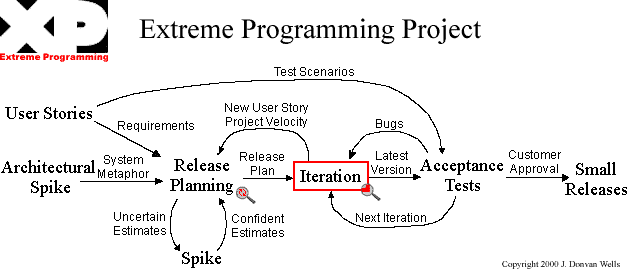
\includegraphics[width=9cm]{images/xp.png}
			\end{center}
			\cite{xpblog}
		}
		}
		
		\hypertarget{uml} {
		\subsubsection{UML: Unified Modeling Language }
		{
			El UML es un lenguaje que permite modelar los elementos que forman un sistema software orientado a objetos, es el lenguaje de modelado mas utilizado en la actualidad aunque aun no es un est�ndar oficial.
			\ds
			Cabe resaltar que UML no es no un m�todo o un proceso, ni una herramienta m�gica que garantiza el �xito del proyecto, sino que es un lenguaje para visualizar de una forma m�s sencilla el proceso del desarrollo.
			\ds
			Dentro de UML podemos encontrar los siguientes diagramas o artefactos:
			\begin{itemize}
			\item Diagrama de clases
			\item Diagrama de componentes
			\item Diagrama de objetos
			\item Diagrama de estructura compuesta
			\item Diagrama de despliegue
			\item Diagrama de paquetes
			\item Diagrama de actividades
			\item Diagrama de casos de uso
			\item Diagrama de estados
			\item Diagrama de secuencia
			\item Diagrama de comunicaci�n
			\item Diagrama de tiempos (UML 2.0)
			\end{itemize}
		}
		}
				
		\hypertarget{refactorizacion} {
		\subsubsection{Refactorizaci�n}
		{
			\textit{$"$ Un cambio hecho a la estructura interna del c�digo para hacerlo m�s f�cil de comprender y m�s barato de modificar sin cambiar su comportamiento externo.$"$}  \cite{refactoring}
			\ds
			En \hyperlink{software}{ingenier�a del software}, el t�rmino refactorizaci�n se usa a menudo para describir la modificaci�n del c�digo fuente sin cambiar su comportamiento, lo que se conoce informalmente por limpiar el c�digo. La refactorizaci�n se realiza a menudo como parte del proceso de desarrollo del software: los desarrolladores alternan la inserci�n de nuevas funcionalidades y casos de prueba con la refactorizaci�n del c�digo para mejorar su consistencia interna y su claridad. Los tests aseguran que la refactorizaci�n no cambia el comportamiento del c�digo.
			\ds
			La refactorizaci�n es la parte del mantenimiento del c�digo que no arregla errores ni a�ade funcionalidad. El objetivo, por el contrario, es mejorar la facilidad de comprensi�n del c�digo o cambiar su estructura y dise�o y eliminar c�digo muerto, para facilitar el mantenimiento en el futuro. A�adir nuevo comportamiento a un programa puede ser dif�cil con la estructura dada del programa, as� que un desarrollador puede refactorizarlo primero para facilitar esta tarea y luego a�adir el nuevo comportamiento.
			\ds
			El termino se refiere a la factorizaci�n matem�tica, para ver una estructura mas clara cuando se realiza esta se realiza. De manera similar, en la refactorizaci�n del software, el cambio en la estructura visible puede frecuentemente revelar la estructura interna $"$oculta$"$ del c�digo original.
			\ds
			La refactorizaci�n debe ser realizada como un paso separado, para poder comprobar con mayor facilidad que no se han introducido errores al llevarla a cabo. Al final de la refactorizaci�n, cualquier cambio en el comportamiento es claramente un error y puede ser arreglado de manera separada a la depuraci�n de la nueva funcionalidad.
			\ds
			Un ejemplo de una refactorizaci�n trivial es cambiar el nombre de una variable para que sea m�s significativo, como una sola letra 't' a 'tiempo'. Una refactorizaci�n m�s compleja es transformar el trozo dentro de un bloque en una subrutina. Una refactorizaci�n todav�a m�s compleja es remplazar una sentencia condicional if por polimorfismo.
			\ds
			Aunque la limpieza de c�digo se lleva realizando desde hace d�cadas, el factor clave de la refactorizaci�n es realizar de manera intencionada la limpieza separ�ndola de la adici�n de funcionalidad nueva, usando un cat�logo conocido de m�todos �tiles de refactorizaci�n, para despu�s comprobar el c�digo ejecutando las pruebas unitarias, sabiendo que cualquier cambio en el comportamiento significa que se ha introducido un error. \cite{wikipedia}
		}
		}
		
		\hypertarget{qt} {
		\subsubsection{Qt}
		{
			La biblioteca fundamental utilizada en este proyecto es Qt, el cual es un \textbf{framework} \hyperlink{multiplataforma}{multiplataforma} r�pido, estable y de r�pida evoluci�n, esta construido sobre el lenguaje de programaci�n \hyperlink{c++}{C++}.
			\begin{center}
			
\includegraphics[width=1.7cm]{images/qt.png}
			\end{center}
			Dentro de sus m�ltiples funcionalidades, Qt permite acceso a componentes gr�ficos y no gr�ficos, y se compone de diferentes m�dulos tales como: core, gui, xml, sql, svg. Cada modulo define un conjunto de clases para acceder a determinadas caracter�sticas.
			\ds
			Qt fue creado por la empresa noruega TrollTech.
		}
		}
		
		\subsubsection{DLib}
		{
			DLib es una extensi�n de \hyperlink{qt}{Qt} que provee componentes gr�ficos y no-gr�ficos de alta calidad, tales como acceso a archivos de configuraci�n automatico utilizando la tecnolog�a \hyperlink{XML}{XML}, \hyperlink{widget}{widgets} para el manejo de fechas, acceso a la \hyperlink{api}{API} de sonido mediante plugins (Actualmente posee un \hyperlink{plugin}{plugin} para \hyperlink{gst}{gstreamer}), entre muchas otras funcionalidades.
			\ds
			DLib fue y sigue siendo programada casi su totalidad por David A. Cuadrado, ha sido el esfuerzo de mucho tiempo por conseguir una extensi�n de \hyperlink{qt}{Qt} \hyperlink{multiplataforma}{multiplataforma}, libre y de f�cil acceso al programador.
		}
			
		\hypertarget{XML} {
		\subsubsection{XML}
		{
			XML (siglas del ingl�s eXtensible Markup Language, lenguaje de marcado extensible) es un lenguaje etiquetas desarrollado por el World Wide Web Consortium (W3C). XML no es un lenguaje predefinido sino un meta-lenguaje que nos permite definir otros lenguajes para usos determinados.
			\ds
			XML es una idea simple pero genial, que puede tener aplicaci�n en cualquier �mbito donde se desee aplicarlo, mediante la especificaci�n de unas etiquetas y su respectiva interpretaci�n mediante analizadores.
			\ds
			Es un excelente m�todo para compartir informaci�n de manera sencilla y r�pida entre diferentes sistemas, entre sus m�ltiples aplicaciones est�n:
			\ds
			\begin{itemize}
			\item Protocolos de comunicaci�n.
			\item Formatos de persistencia.
			\item Aplicaciones en el web.
			\item Archivos de configuraci�n.
			\item Bases de datos.
			\end{itemize}
			\textbf{Historia} \\
			La historia del XML comienza en los a�os 70, cuando IBM crea un lenguaje llamado GML ( de las siglas en ingl�s, General Markup Language), esta empresa utilizo este lenguaje para el almacenamiento de grandes cantidades de datos, debido a su f�cil y r�pida capacidad de acceso a los datos.
			\ds
			Despues de que IBM liberar� la especificaci�n de este lenguaje, la ISO decidi� normalizarlo en lo que hoy se conoce como SGML (Standard General Markup Language) en el a�o de 1986.
			\ds
			Basado en este lenguaje, en 1989 se crea una especificaci�n llamada HTML (HiperText Markup Language) utilizado en el WWW (World Wide Web), desafortunadamente HTML creci� desmedidamente y algunas empresas como Microsoft y Netscape decidieron incluir etiquetas incompatibles con el est�ndar, es as� como en 1998 el consorc�o empez� a desarrollar XML, con el fin de reemplazar HTML.
			\\
			\ds
			\textbf{Objetivos} \\
			Este lenguaje fue creado para cumplir b�sicamente los siguientes objetivos:
			\begin{itemize}
			\item {Ser compatible con HTML.}
			\item Consistencia en el tratamiento de los datos.
			\item General y extensible.
			\item F�cil modificaci�n y lectura.
			\item F�cil implantaci�n.
			\end{itemize}
			\textbf{Ventajas} \\
			\begin{itemize}
			\item Permite hacer traducciones a otros formatos f�cilmente, esto facilita la comunicaci�n entre aplicaciones.
			\item La interpretaci�n de un documento XML es sencilla y r�pida.
			\item El acceso a los datos alojados en el documento es r�pido gracias a su forma de �rbol.
			\end{itemize}
		}}
		
		\hypertarget{modelo_colaborativo} {
		\subsubsection{Modelos colaborativos}
		{
			Trata de aplicar el dicho popular \textit{"la uni�n hace la fuerza"} a la inform�tica, mediante la combinaci�n de equipos de computo para lograr un fin com�n. \\
			Mediante este modelo se aumenta la productividad y la eficiencia en los procesos de producci�n.
			Para que el modelo funcione, es necesario que los componentes tengan la mentalidad y el deseo de cooperar en busca del bien com�n. \\
			\ds
			\textbf{Sinergia} \\
			La sinergia es la combinaci�n de diversos elementos para lograr un beneficio mayor, en esta teor�a la combinaci�n de las partes es mayor a la suma de las partes, es decir, se obtiene un beneficio mayor al trabajo de las partes independientemente. \\
			\ds
			\textbf{La sinergia en la teor�a general de sistemas} \\
			Al analizar las partes de un sistema de manera individual, cada parte no es capaz de dar informaci�n relevante sobre las caracter�sticas de �l mismo, entonces decimos que es un componente sin�rgico. Cada sistema sin�rgico, esta compuesto de otros sistemas tambi�n sinergicos.
		}}
		
		\hypertarget{c++} {
		\subsubsection{C++}
		{
			C++ es una extensi�n de C, b�sicamente para soportar objetos de forma directa, fue dise�ado por Bjarne Stroustrup en los a�os '80.
			\ds
			Dentro de sus caracter�sticas principales tenemos:
			\begin{itemize}
			\item Soporte Programaci�n Orientada a Objetos (POO).
			\item Soporte para plantillas, las cuales aseguran la generalidad de la clase.
			\item Soporte para excepciones en tiempo de ejecuci�n.
			\item Soporte para sobrecarga de operadores, tales como la suma, resta, indexaci�n.
			\item Identificaci�n de tipos en tiempo de ejecuci�n.
			\end{itemize}
			En 1983, Rick Masiatti propuso el nombre de C++, haciendo aluci�n a la instrucci�n valida c++, que significa aumentar en 1 el valor de la variable C, esto significa que es el siguiente paso de C.
			\ds
			C++ es un lenguaje muy potente y robusto, permite trabajar en alto y bajo nivel. Adem�s, esta estandarizado y por tanto permite implementarse en cualquier plataforma.
		}}
		
		\hypertarget{SMIL} {
		\subsubsection { SMIL }
		{
			SMIL (pronunciado ESMAIL), es una opci�n libre, abierta y est�ndar al formato SWF de \hyperlink{flash}{Macromedia Flash} creada por el W3C, fue recomendado en diciembre de 2005.
			El objetivo principal de este est�ndar es definir una lenguaje basado en \hyperlink{XML}{XML} para crear contenido multimedia, sincronizando m�ltiples elementos como audio, v�deo y lo mas importante, im�genes vectoriales descritas por el est�ndar \hyperlink{svg}{SVG}. \cite{smil}
		}}
		
		\hypertarget{svg} {
		\subsubsection { SVG }
		{
			Scalable Vector Graphics (SVG) es una especificaci�n de \hyperlink{XML}{XML} utilizado para describir \hyperlink{graficos_vectoriales}{gr�ficos vectoriales}, con posibilidad de animarlos.
			Es un est�ndar de la W3C, fue recomendado en el 2001 y desde esa fecha se ha extendido mucho, en este momento muchos navegadores lo incluyen de manera nativa dentro del n�cleo de renderizado. \\
			\ds
			\textbf{Caracter�sticas} \\
			SVG permite combinar im�genes, gr�ficos vectoriales y texto en un mismo archivo, y sobre estos componentes se permite realizar transformaciones y composiciones. Adem�s tambi�n se puede aplicar efectos a los objetos componentes.
			\ds
			Una caracter�sticas importante y poco explotada de los SVG es la capacidad de ser interactivos, mediante el uso de scripts es posible a�adir eventos tales como \textit{onclick}, \textit{onmouseover}, a las animaciones creadas en este formato2. \cite{svg}
		}
		}
		
		\hypertarget{proceso_de_animacion}{
		\subsubsection{El proceso de animaci�n tradicional}
		{
			\comillas{La animaci�n tradicional es un proceso costoso, que consume mucho tiempo.} \cite{hollywood}
			\begin{center}
			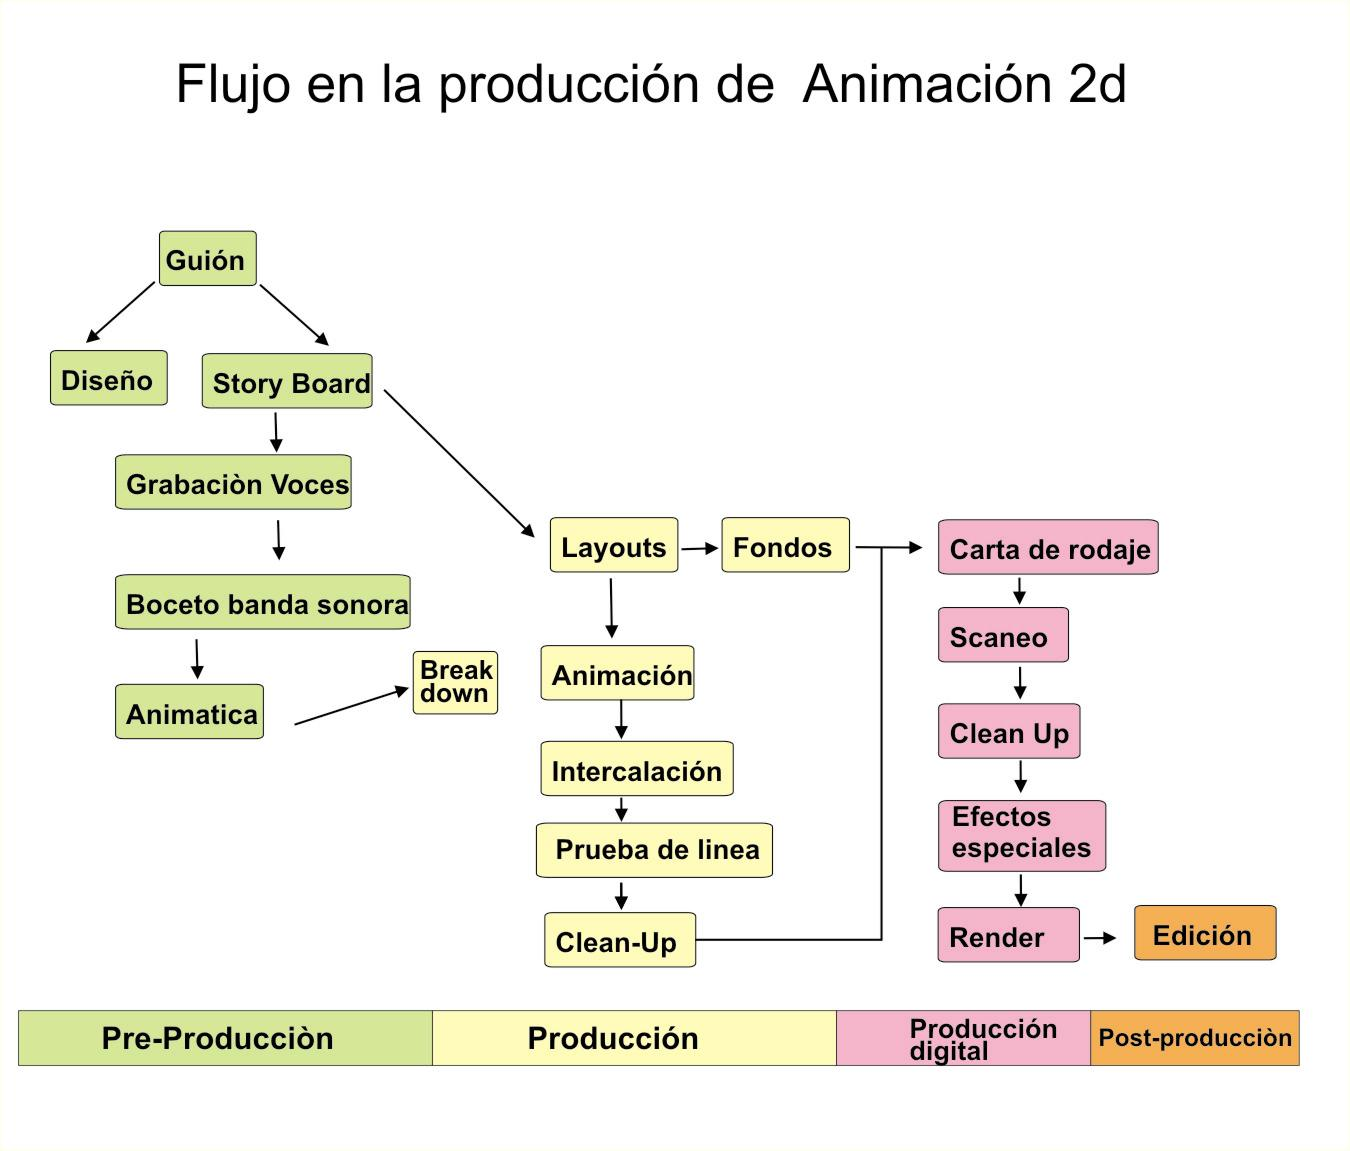
\includegraphics[width=12cm]{images/animacion2d.png}
			\end{center}
			\textbf{PRE-PRODUCCI�N} \\
			Igual que todos los procesos, la animaci�n empieza con una idea que puede surgir en cualquier momento y en cualquier lugar. El concepto de la animaci�n debe ser pensado al interior del estudio y el escritor debe dar luz verde para la realizaci�n. \\
			Antes o despues de que el script es terminado, la empresa debe buscar un director para ese proyecto. El director ser� quien vigile todos los aspectos de la creaci�n, es por eso que cada artista tiene que participar en el proceso con el director. \\
			El tiempo usado por el director en estas semanas de pre-producci�n es bastante, buscando artistas, repartiendo trabajos y en general prepar�ndose para la etapa de producci�n. \\
			Una vez el script esta escrito, el equipo de aristas comienza a trabajar en el desarrollo visual. \\
			\\
			\textbf{Dise�os de personajes}
			\\
			\\
			El Director realizar� o designar� un artista para la confecci�n de los dise�os de personajes. \\
			\begin{itemize}
			\item Cuando el mismo director realiza los dise�os de personajes, por lo general los hace al un�sono con los dise�os de escena.
			\item Los dise�os de personajes deben contener: \\
			Todos los dise�os de personajes principales, secundarios y extras, con su frente,   espalda, tres cuartos y perfil, en caso de que se necesitaran todas estas posiciones. Tama�o de los personajes y estados comparativos de proporciones.
			\end{itemize}
			El tiempo y pago de esta etapa se considerar� a partir de una propuesta conjunta entre el Director y el Productor y elevada a la instancia del Sub director de producci�n para su aprobaci�n.
			\\
			\textbf{Dise�os de escena y layouts} \\
			El Director puede hacer o designar a otro artista para que realice esta etapa.
			\begin{itemize}
			\item Esta etapa debe contener a su terminaci�n: \\
			Dise�os de personajes con todos los elementos se�alados en la etapa de dise�os de personajes.
			\end{itemize}
			\begin{center}
			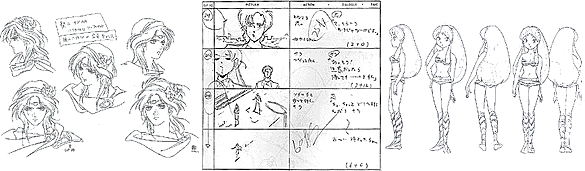
\includegraphics[width=10cm]{images/preproduccion.png}
			\end{center}
			\textbf{PRODUCCI�N} \\
			\textbf{Presupuesto y cronograma del proyecto} \\
			\\
			Con cada una de estas figuras art�sticas se reunir�an el Director y el Productor para acordar tiempos de realizaci�n (cronograma por etapas), formas de pagos y discusi�n art�stica t�cnica del proyecto. Estas reuniones individuales y colectivas estar�an a cargo del Productor. \\
			\\
			La propuesta  de la confecci�n  de cada uno de estos equipos ser�a seleccionada por cada uno de ellos, de acuerdo con el Productor y El Director y tomando en cuenta las necesidades, prioridades y problem�tica del estudio en ese momento particular. \\
			\\
			Elaborado el presupuesto y el cronograma se elevar�a a la Direcci�n del estudio para su aprobaci�n final. De existir discrepancias en torno a los mismos, se reunir�an El Director y el Productor con esta instancia para reajustar o dar sus criterios en los casos necesarios. \\
			\\
			Aprobado  el proyecto, la subdirecci�n de producci�n har�a el cronograma final  de comienzo y termino. \\
			\\
			\textbf{Grabaci�n de voces} \\
			Luego de confeccionados y revisados los di�logos, el productor coordinar� la grabaci�n de los mismos con el estudio de sonido, y se ocupar� de todos los factores implicados en el llamado para cumplir con esta etapa. \\
			Grabados los di�logos,  el productor coordinar� un llamado para que el Director, el Editor, y el Director de Animaci�n ajusten los mismos y se pueda proceder a la etapa de la Direcci�n de Animaci�n. \\
			\\
			\textbf{Etapa de animaci�n} \\
			Luego de realizada la primera Etapa de la direcci�n de animaci�n se reunir�a el Director de Animaci�n con su equipo para comenzar la animaci�n del filme. Estas reuniones preliminares a la animaci�n deben incluir una reuni�n con  el  Director de Fotograf�a  y el equipo de Infograf�a, para dudas, aportes y cualquier dato importante que sea necesario para el trabajo entre ellos. \\
			\\
			Terminada esta primera etapa de la Direcci�n de Animaci�n, se comenzar� la animaci�n del proyecto seg�n el cronograma establecido, la cu�l estar� regida art�sticamente por el Director de Animaci�n y controlada por el productor, para que se cumpla en tiempo y con calidad todo el proceso. Ser� de la competencia del productor coordinarles al Director de Animaci�n y al Director el visionaje de la animaci�n. \\
			\\
			Tratar de que finalizada la etapa de animaci�n se pueda visionar la misma con las voces sincronizadas, para evitar ajustes posteriores en la etapa de edici�n. \\
			\\
			\textbf{Infograf�a: Album de color.}
			El Director y la colorista definen el color de los personajes y los props y models  necesarios para el proyecto en cuesti�n. El Director de fotograf�a debe tener un visionaje de todos estos elementos junto con los fondos para definir con el Director la l�nea art�stica  que finalmente tendr� el proyecto, y as� evitar errores posteriores. \\
			\\
			El proyecto podr�a entrar en la etapa de infografia completo o por etapas, en dependencia de las necesidades de producci�n del estudio. \\
			\\
			El Director, el Director de Animaci�n, y el editor deben estar al tanto del proyecto mientras est� en esta etapa, as� como atender cualquier solicitud del Director de Fotograf�a en aras de solucionar en ese momento cualquier problema que pueda surgir. \\
			\\
			Finalizado el proyecto en Infograf�a se har� un visionaje total del mismo con el grupo art�stico para dar la aprobaci�n final a la etapa. \\
			\\
			Despu�s de  definir todos los aspectos art�sticos del proyecto, se procede a animar cuadro a cuadro en las mesas de  animaci�n, este proceso se divide entre el animador principal que define las poses claves, el intercalador, que interpreta los movimientos entre cuadros claves y  los limpiadores ( Cleanup ) y coloristas de la animaci�n que utilizan las im�genes escaneadas programa de animaci�n para  pasar estas im�genes a arte vectorial.
			\begin{center}
			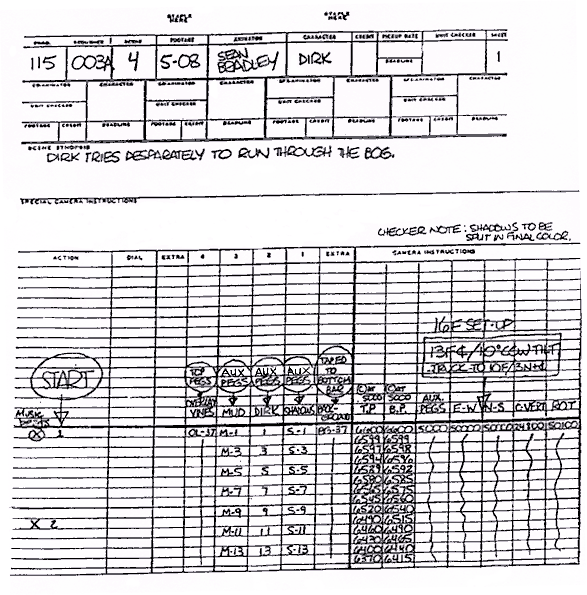
\includegraphics[width=10cm]{images/exposure_sheet.png} \\
			Tabla de exposici�n
			\end{center}
			\textbf{POST-PRODUCCI�N} \\
			Esta etapa necesita y se nutre de los siguientes factores. \\
			\\
			\begin{itemize}
			\item Imagen sincr�nica con las voces (en caso de tenerlas)
			\item Tener el primer corte de imagen aprobado por el Asesor.
			\item Trabajo coordinado con el estudio de sonido para la b�squeda de los elementos sonoros necesarios para la confecci�n de la banda sonora.
			\item Grabaci�n de efectos sonoros (caso de necesitarlos)
			\item Visionaje con m�sico: Realizaci�n de la m�sica y aprobaci�n.
			\item Composici�n de todos los planos de la animaci�n en un programa de v�deo
			\item Efectos visuales de la animaci�n en un programa de v�deo
			\item Mezcla final. Visionaje con el Asesor.
			\item Visionaje en sala con la direcci�n de los Estudios.
			\item Edici�n final de la animaci�n
			\item Transfer
			\item Visionaje en sala con el equipo de la pel�cula.
			\end{itemize}
		}
	}
	
	\subsection{Antecedentes}
	{
		A pesar de que no se encontraron trabajos similares al planteado, no se
		descarta la posibilidad de que exista software con las caracter�sticas propuestas en este
		proyecto.
		\ds
		No obstante, se pueden presentar dos herramientas comerciales que sirven
		para realizar animaciones, que de alguna manera involucran aspectos relacionados con la producci�n de animaciones.
		
		\hypertarget{flash} {
		\subsubsection{Macromedia Flash}
		{
			Es una herramienta de la empresa Macromedia para la creaci�n de contenido multimedia, por ende permite combinar en una misma presentaci�n v�deo, audio y texto, con soporte total para eventos.
			\ds
			Flash puede llegar a ser todo un lenguaje de programaci�n, sinembargo la parte de inter�s para este proyecto esta en la capacidad para realizar animaciones sobre este software tan utilizado a nivel mundial.
			\ds
			Esta es una de las herramientas mas usadas y populares a nivel mundial debido a que es muy potente y poco a poco se ha convertido en una herramienta de uso extendido en la industria de la animaci�n y la multimedia.
		}}
		\subsubsection{ToonBoom}
		{
			A diferencia de Macromedia Flash, ToonBoom es una aplicaci�n �nicamente destinada a la creaci�n de animaciones. \\
			Esta aplicaci�n esta programada con las bibliotecas \hyperlink{qt}{Qt}, es un software muy potente ampliamente utilizado por empresas dedicadas a la creaci�n de contenido animado a nivel mundial.
		}
		
		Una de las caracter�sticas mas extra�adas de estas herramientas es un servidor que mantenga las bibliotecas para que el equipo de animaci�n pueda acceder f�cilmente a �l trabajo de sus compa�eros, este proyecto pretende cubrir este agujero.
	}
	
	\subsection{Marco conceptual}
	{
		A continuaci�n se presentan una serie de conceptos clave o referenciados en este proyecto.
		
		\subsubsection{Conceptos relacionados con la inform�tica}
		{	
			\begin{itemize}
			\hypertarget{multiplataforma} {
			\item{\textbf{multiplataforma} } \\
			Propiedad del software que le permite ejecutarse en varias plataformas. Normalmente las plataformas se refieren a GNU/Linux, Mac Os X y Microsoft Windows.
			}
			\hypertarget{graficos_vectoriales} {
			\item {\textbf{Gr�ficos vectoriales}} \\
			Son gr�ficos a los que se les pueden aplicar operaciones sin que ello empeore la calidad.}
			\hypertarget{plugin}{
			\item { \textbf{Plugin }} \\
			Programas que pueden ser cargador en tiempo de ejecuci�n por otras aplicaciones.
			}
			\hypertarget{gst}{
			\item{ \textbf{GStreamer }} \\
			GStreamer es un framework para crear aplicaciones multimedia. GStreamer hace posible escribir cualquier aplicaci�n multimedia debido a su alta generalidad, facilidad de acceso y su rapidez. Adem�s este framework es \hyperlink{multiplataforma}{multiplataforma}.
			}
			\hypertarget{widget} {
			\item{\textbf{Widget}} \\
			Componente esencial y b�sico de una interfaz gr�fica de usuario.
			}
			\hypertarget{api} {
			\item{\textbf{API}} \\
			M�todo de acceso a la interfaz de programaci�n, ayuda al programador a realizar mas f�cilmente sus tareas y de forma mas organizada, permitiendo el acceso a los diferentes componentes de una biblioteca.
			}
			\hypertarget{user_stories} {
			\item{\textbf{User stories}} \\
			Describen el caso de uso en t�rminos del cliente, \comillas{user} en este caso se refiere al cliente.
			}
			\end{itemize}
		}
		
		\subsubsection{Conceptos relacionados con la animaci�n}
		{
		\begin{itemize}
		
		\item \textbf{Anim�tica} \\
		Conocida tambi�n como tira leica o leica reel, es la grabaci�n y edici�n de las im�genes del \hyperlink{story_board}{Story Board} sincronizada con la banda sonora y el audio de los personajes, con esta ficha es posible controlar los tiempos de la animaci�n y entender en movimiento lo visualizado en el papel para corregir errores de ritmo poder generar una idea de como ser� la pel�cula al final.
		
		\item \textbf{Backgrounds} \\
		Fondos o escenograf�as de la animaci�n.
		
		\item \textbf{Ciclo }
		Secuencia de animaci�n repetitiva para mostrar una acci�n como la de caminar o correr.
		
		\item \textbf{Biblia} \\
		El Universo del proyecto de animaci�n que contiene, el concepto, sinopsis  de los cap�tulos y el dise�o del personaje con indicaciones de c�mo dibujarlo y animarlo.
		
		\hypertarget{exposure} {
		\item \textbf{Hola de exposici�n (Exposure Sheets)} \\
		Hoja de exposici�n o la carta de rodaje donde se consigna con detalle cada uno de los cuadros que intervienen en una acci�n.
		}

		\item \textbf{Extremo}\\
		Dibujo final, al final de una pose.
		
		\hypertarget{frame} {
		\item \textbf{Marco (frame)} \\
		Es la unidad de una secuencia de animaci�n, en la televisi�n 30 frames componen un segundo de animaci�n.
		}
		
		\hypertarget{layer} {
		\item \textbf{Capa (layer)} \\
		Es la agrupaci�n de marcos o frames.
		}
		
		\hypertarget{scene} {
		\item \textbf{Plano o escena (scene)} \\
		Es la agrupaci�n de fotogramas.
		}
		
		\hypertarget{gc} {
		\item \textbf{Componente gr�fico} \\
		Es un objeto individual que representa un componente de un marco o frame.
		}
		
		\item \textbf{Giros}\\
		Las vistas frontales, laterales y de espaldas de un personaje permitiendo visualizar una imagen tridimensional del personaje.
		
		\hypertarget{script} {
		\item \textbf{Gui�n} \\
		En ingles llamado \textit{script} que es el desarrollo escrito de la acci�n, di�logo y  los sonidos de una animaci�n
		}
		
		\hypertarget{hoja_modelo} {
		\item \textbf{Hoja de Modelo} \\
		Gu�a que representa todas las posiciones de las vistas girando en 360�, los detalles, y las diferentes poses, expresiones y estados de �nimo.
		}
		
		\hypertarget{intercalado} {
		\item \textbf{Intercalado} \\
		Tambi�n se llaman Intermedios o Inbetwenner, que son la cantidad de  dibujos que unen las puntas o dibujos claves en una animaci�n 
		}
		
		\item \textbf{Key}\\
		Es un dibujo clave representado por una pose importante en la animaci�n.
		
		\item \textbf{Layout} \\
		Es  la  planeaci�n gr�fica de un plano de animaci�n, donde se visualiza la composici�n b�sica y los movimientos de  una c�mara.
		
		\item \textbf{Animaci�n Limitada} \\
		La Animaci�n limitada es la industrializaci�n de la animaci�n, muy com�n en televisi�n donde se consumen series r�pidamente
		
		\item \textbf{Lip-sync} \\
		Es la \textit{sincronizaci�n} del audio con las im�genes. Y la descomposici�n del di�logo (fonemas) y la  m�sica en cuadros para acoplar imagen y audio.
		
		\item \textbf{Mesa de animaci�n} \\
		Mesa de luz donde se trabajan los fotogramas de una animaci�n, utilizando hojas de papel delgado, aprovechando las transparencias que deja la luz para visualizar el movimiento de la animaci�n.
		
		\item \textbf{Prueba de L�nea} \\
		Filmaci�n de la animaci�n en su primera etapa de realizaci�n. Llamada tambi�n \textit{Prueba de l�piz en 2D}.
		
		\hypertarget{story_board} {
		\item \textbf{Story-board} \\
		Dibujos en forma de historieta de todo el desarrollo de la pel�cula, acompa�ado de los textos que explican las acciones y los di�logos de las escenas.
		}
		
		\hypertarget{timming} {
		\item \textbf{Timming} \\
		Ritmo. Visualizaci�n de los tiempos en animaci�n.
		}
		
		\hypertarget{tweening} {
		\item \textbf{Interpolaci�n (Tweening)} \\
		Dibujar dos o mas elementos (manos, brazos, piernas...) repitiendo la misma acci�n al mismo tiempo
		}
		
		\end{itemize}
		}
		\subsubsection{Roles}
		\begin{itemize}
		\item \textbf{ Creador Original} \\
		El creador Original es la persona que plantea el concepto original de la historia, la base de la creaci�n. Puede ser un director, productor, ilustrador, novelista, o guionista. 

		\item \textbf{Productora} \\
		Es la compa��a que acoge el proyecto y decide invertir tiempo, dinero y recursos en todas las fases de la producci�n.
		
		\hypertarget{director} {
		\item \textbf{Director} \\
		El Director es el responsable de todo  el desarrollo visual, art�stico y audiovisual del Proyecto. Es el l�der de la animaci�n  y determina el tipo de producci�n  que se desea realizar, visualiza el story board que son los dibujos detallados de las secuencias de animaci�n y  maneja toda la informaci�n que tiene que ver con el di�logo, la m�sica, el ritmo y el trabajo de c�mara.
		}
		
		\item \textbf{Productor} \\
		Es la persona encargada de coordinar y seguir todas las tareas de de las personas involucradas en la producci�n, maneja los cronogramas y el presupuesto detallado y junto al director decide  cosas importantes que ata�en a la producci�n.
		
		\hypertarget{director_animacion} {
		\item \textbf{Director de Animaci�n} \\
		Es un rol que esta entre el \hyperlink{director}{director} y la producci�n, es el responsable de liderar el estilo de animaci�n y de revisar y supervisar la producci�n de todo el show desde la historia inicial, hasta la postproducci�n final.
		�l revisa los dibujos hechos por el equipo de animaci�n y visualiza el m�todo para realizar estas \hyperlink{scene}{escenas}.
		}
		
		\item \textbf{Dise�ador de Personajes} \\
		Esta persona hace parte del equipo creativo de la producci�n y se involucra desde la pre-producci�n desarrollando todo el dise�o de los personajes para el proyecto. Este integrante del equipo provee una Biblia del proyecto con toda la informaci�n gr�fica de los personajes, detalladas en poses, gestos y construcci�n del personaje.
		
		\item \textbf{Animadores Clave} \\
		El animador clave trabaja desde el \hyperlink{story_board}{story board}  y crea las \hyperlink{scene}{escenas} claves de la animaci�n, las posiciones del personaje, la integraci�n con los fondos y determina el \hyperlink{timming}{ritmo} y la cantidad de \hyperlink{frame}{frames} asociados en el movimiento.
		
		\item \textbf{Intercalador} \\
		El  intercalador usa los cuadros claves de la animaci�n como punto referencial para desarrollar los \hyperlink{frame}{cuadros} restantes, estos cuadros permiten generar una animaci�n mas fluida y  profesional. El intercalador no es un trabajo creativo y requiere much�simas horas de trabajo.
		
		\item \textbf{Clean Up} \\
		Como el intercalador es un trabajo que requiere muchas horas y se   encarga de darle detalle a la l�nea y de colorear todos los cuadros de la animaci�n.
		
		\item \textbf{Storyboarder} \\
		Es el ilustrador encargado de plasmar en dibujos cada uno de los planos de la animaci�n, por lo regular es el mismo director o el creador de los personajes del proyecto.

		\end{itemize}
	}
}


\section{Aspectos Metodol�gicos}
{
	\subsection{Tipo de Proyecto y Justificaci�n de su Magnitud }
	{
		Fundamentalmente el proyecto es de tipo pr�ctico, con algunos aspectos investigativos, al final del proceso se entregara una herramienta con las funcionalidades propuestas, debido a la magnitud de los sub-productos que ser�n entregados son necesarias dos personas para realizar este trabajo de grado.
	}
	
	\subsection{Resultados esperados}
	{
		\begin{itemize}
		\item Una aplicaci�n servidor que servira para gestionar y centralizar la informaci�n.
		\item Un cliente que permita realizar animaciones y pueda usar el servidor como medio de gesti�n.
		\item Un cliente administrador que permita gestionar diferentes aspectos del sistema.
		\item Un documento que contenga el est�ndar de comunicaci�n con el servidor.
		\item C�digo fuente y ejecutable de las aplicaciones y bibliotecas desarrolladas en el proyecto, artefactos de an�lisis y de dise�o generados, documentaci�n interna.
		\end{itemize}
	}
	
	\subsection{Metodolog�a de desarrollo}
	{
		Para el desarrollo del proyecto se usara un proceso �gil, para esto se ha elegido la metodolog�a \hyperlink{xp}{\textit{Programaci�n Extrema}}, en combinaci�n con algunos artefactos propios de \hyperlink{uml}{\textit{UML}}.
		\ds
		El enfoque elegido nos permitir� definir unas caracter�sticas b�sicas de versiones a corto plazo, con la idea de implementar y corregir un conjunto de peque�os avances.
	}
	
	\subsection{Plan de Actividades}
	{
		La \hyperlink{xp}{Programaci�n Extrema} se compone de 4 fases importantes, que son: \textbf{plan, dise�o, codificaci�n y pruebas}, pero estas fases no se realizan de forma completa y en orden, sino que cada una se compone de actividades que se van desarrollando de manera iterativa e incremental.
		
		\subsubsection{Fase de planeaci�n}
		{
			\begin{itemize}
			\item Escribir el documento de anteproyecto de grado.
			\item Cada iteraci�n empieza con un plan, donde se escriben las tareas que cada iteraci�n debe cumplir.
			\item Analisis de riesgos.
			\end{itemize}
		}
		\subsubsection{Fase de dise�o}
		{
			\begin{itemize}
			\item Escribir el est�ndar de codificaci�n.
			\item Escribir las pol�ticas de uso del servidor de control de versiones.
			\item Por cada iteraci�n, realizar \hyperlink{refactorizacion}{refactorizaci�n} cuando sea necesario.
			\item Dise�o de pruebas.
			\item Definici�n de arquitectura y m�dulos.
			\end{itemize}
		}
		
		\subsubsection{Fase de codificaci�n}
		{
			\begin{itemize}
			\item Implementaci�n con avances r�pidos y optimizaciones al final.
			\item Codificaci�n de pruebas.
			\item Documentaci�n de usuario.
			\item Documentaci�n interna.
			\end{itemize}
		}
		
		\subsubsection{Fase de pruebas}
		{
			\begin{itemize}
			\item Aplicaci�n de pruebas unitarias.
			\item Cuando se encuentra un error de codificaci�n o de l�gica, se desarrollan pruebas para evitar volver a caer en el mismo.
			\end{itemize}
		}
		
		
		La documentaci�n de la tesis ser� una actividad que se desarrollara a lo largo de todo el proyecto y paralelo a las dem�s actividades.
	}
}


\section{Cronograma}
{

}


\section{Aspectos administrativos}
{

}

\section{Aspectos financieros}
{
	En la presente secci�n, se muestra un presupuesto estimada para el proyecto.
	\subsection{Presupuesto}
	{
		\begin{center}
		\begin{tabular}[c]{|l|l|l|l|l|l|}
			\hline
			\textbf{ITEM} & \textbf{ESFUERZO}  & \textbf{VALOR HORA} & \textbf{CONCEPTO} & \textbf{APORTES} & \textbf{VALOR}  \\
			\hline
			1.  	& 		&	& Personal 		&		& 	\\
			1.1.  	& 	640	&	\$10.000=	& Desarrolladores 	&		& 	\$6'400.000= \\ 
			1.2.  	& 	320	&	\$20.000= & Director de tesis 	&	\$6'400.000=	& 	 \\ 
			1.3.  	& 	40	&	\$20.000= & Asesores 		&		& 	\$800.000= \\ 
			1.4.  	& 	40	&	\$5.000= & Personal experto 	&		& 	\$200.000= \\
			\hline
			2. 	& 		&	& Equipo de oficina 	&		& 	\\ 
			2.1.  	& 	480	&	\$2.000= & Equipos de computo 	&	\$480.000=	& 	\$480.000= \\ 
			2.2.  	& 		&	& Documentaci�n 		&		& 	\$300.000= \\ 
			2.3.  	& 		&	& CD's y DVD's 		&		& 	\$50.000= \\ 
			\hline
			3.  	& 		&	& Generales 		&		& 	\\
			3.1	&	320	&	\$2.500= & Telecomunicaciones	&	\$400.000=	&	\$400.000= \\
			3.2.  	& 		&	& Vi�ticos 		&		& 	\$1'440.000= \\ 
			4.  	& 		&	& Imprevistos 		&		& 	\$500.000= \\
			\hline
				&&&	SUBTOTAL		&	\$7'280.000= &	\$10'570.000= \\
			\hline
			\hline
				&&& 	TOTAL 			&&	\$17'850.000 \\
			\hline
		\end{tabular}
		\end{center}
		
		
		\textbf{NOTAS}
		\begin{itemize}
		\item El esfuerzo esta medido en horas.
		\item El presupuesto fue estimado sobre un tiempo de 8 meses.
		\item Los aportes se refieren al valor directo o indirecto que aporta la universidad del valle al proyecto.
		\end{itemize}
	}
}



\bibliography{bibliografia}

\end{document}

